\documentclass[12pt,a4paper]{article}
\usepackage[T1]{fontenc}
\usepackage[utf8]{inputenc}
\usepackage[english,spanish]{babel}
\usepackage[margin=2.5cm]{geometry}
\usepackage{amsmath,booktabs,listings,graphicx,tikz}
\usepackage[backend=biber,style=ieee]{biblatex}
\addbibresource{referencias.bib}
\usepackage{hyperref}
\title{Práctica experimental U1: sockets TCP, gRPC y relojes de Lamport}
\author{Integrante 1 \and Integrante 2 \and Integrante 3 \and Integrante 4}
\date{Fecha pendiente}
\begin{document}
\maketitle
\noindent Código de actividad: GA-SUM-02 / PE-U1. URL pública: \url{https://github.com/BelindaTZ/GA-SUM-02-PE-U1}.
\newpage
\section*{Estado de esta plantilla}
Documento inicial sin resultados. Completar con trabajo y mediciones reales.
Adaptar a la plantilla institucional y alcanzar diez páginas de contenido sin portada ni bibliografía.
\section*{Resumen}
Pendiente: resumen en español y palabras clave; aclarar extensión de 200 palabras.
\begin{otherlanguage}{english}
\section*{Abstract}
Pending: English abstract and keywords.
\end{otherlanguage}
\section{Objetivo e hipótesis}
Registrar hipótesis antes de medir.
\section{Fundamento teórico}
\subsection{Sistemas distribuidos, transparencias ANSA y CAP}
Pendiente.
\subsection{Sockets TCP/UDP, RPC, gRPC, Protocol Buffers y RMI}
Pendiente.
\subsection{Lamport, relojes vectoriales y causalidad}
Pendiente.
\subsection{Fallos y seguridad}
Pendiente: clasificación de fallos, detección, recuperación, JWT y OAuth 2.0.
\section{Arquitectura}
Pendiente: diagrama TikZ de la arquitectura de tres nodos y contrato proto.
% Al existir el archivo: \lstinputlisting{../proto/messaging.proto}
\section{Implementación}
Pendiente: decisiones, framing TCP, acuses, concurrencia y fragmentos breves de código real.
\section{Protocolo experimental}
Pendiente: máquina, versiones, tamaños, repeticiones, calentamiento y criterios de errores.
\section{Resultados}
Pendiente: importar tablas y gráficos producidos por el script.
% Ejemplo futuro: % Generado por analysis/analyze.py. No editar a mano.
\begin{table}[htbp]
\centering
\caption{Latencia RTT por modo, mecanismo y tamaño (sin calentamiento, solo status=ok)}
\label{tab:latencia}
\resizebox{\linewidth}{!}{%
\begin{tabular}{lllrrrrrrr}
\toprule
Modo & Mecanismo & Bytes & Corridas & n & Media (ms) & Mediana (ms) & Desv. (ms) & p95 (ms) & IC95 $\pm$ (ms) \\
\midrule
concurrent & grpc & 100 & 5 & 500 & 2.358 & 2.307 & 0.590 & 3.456 & 0.286 \\
concurrent & grpc & 10240 & 5 & 500 & 2.560 & 2.512 & 0.613 & 3.623 & 0.184 \\
concurrent & sockets & 100 & 5 & 500 & 1.637 & 1.615 & 0.466 & 2.404 & 0.078 \\
concurrent & sockets & 10240 & 5 & 500 & 1.984 & 1.938 & 0.577 & 3.007 & 0.129 \\
sequential & grpc & 100 & 5 & 500 & 1.013 & 0.989 & 0.170 & 1.264 & 0.057 \\
sequential & grpc & 10240 & 5 & 500 & 0.913 & 0.893 & 0.084 & 1.095 & 0.040 \\
sequential & sockets & 100 & 5 & 500 & 0.632 & 0.618 & 0.080 & 0.774 & 0.041 \\
sequential & sockets & 10240 & 5 & 500 & 0.785 & 0.775 & 0.131 & 0.975 & 0.068 \\
\bottomrule
\end{tabular}%
}
\end{table}

% Ejemplo futuro: 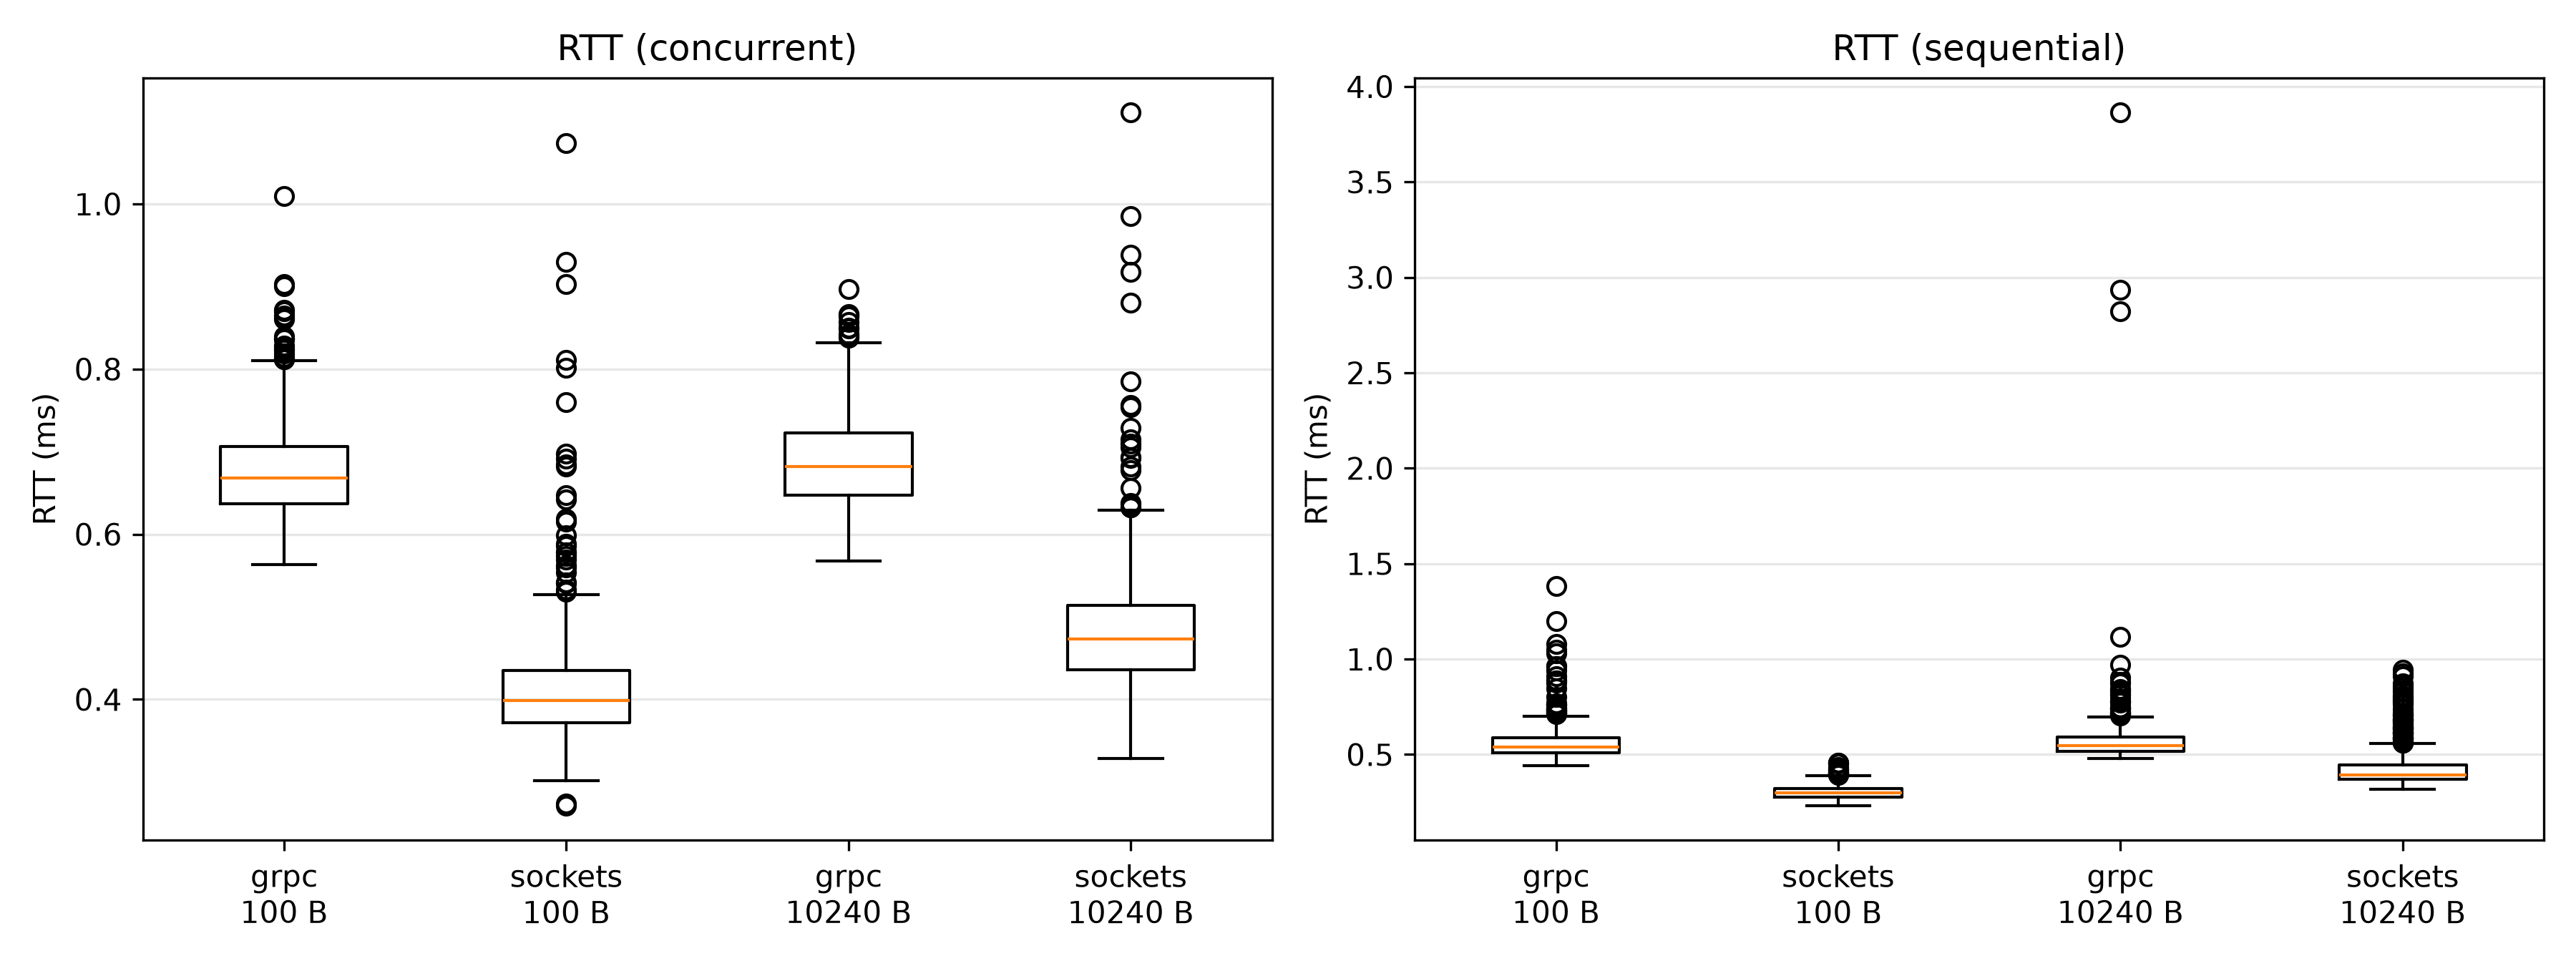
\includegraphics[width=\linewidth]{figures/boxplot.png}
\section{Discusión}
Pendiente: hipótesis, latencia, variabilidad, rendimiento, tipado, desarrollo, errores, PFC y validez.
\section{Verificación de Lamport}
Pendiente: comprobación de datos reales, desigualdad envío/recepción y concurrencia.
\section{Preguntas obligatorias de la guía}
Pendiente: ANSA, caída de nodo, elección para el PFC desde CAP y efecto del número de nodos.
\section{Conclusiones cuantificadas}
Pendiente: afirmaciones respaldadas por mediciones reales.
\subsection{Conclusión individual: integrante 1}
Pendiente: al menos 150 palabras escritas por el integrante.
\subsection{Conclusión individual: integrante 2}
Pendiente: al menos 150 palabras escritas por el integrante.
\subsection{Conclusión individual: integrante 3}
Pendiente: al menos 150 palabras escritas por el integrante.
\subsection{Conclusión individual: integrante 4}
Pendiente: al menos 150 palabras escritas por el integrante.
\section{Aportes y autoría}
Pendiente: tabla de aportes con enlaces a commits reales.
\section{Declaración de uso de inteligencia artificial}
La organización inicial del repositorio y esta plantilla se prepararon con asistencia de IA.
El equipo debe revisar esta declaración y detallar las herramientas, usos y verificaciones efectivamente realizados.
\printbibliography[title={Referencias}]
\end{document}
